\documentclass[aspectratio=169, 13pt]{beamer}
\usepackage[utf8]{inputenc}
\usepackage[english,russian]{babel}
\usepackage{graphicx}
\usepackage{sidecap}
\usepackage{mathtools}
\usepackage{bbm}
\usepackage{appendixnumberbeamer}

\newcommand{\sbrkt}[1]{\left[ #1 \right]}
\DeclarePairedDelimiter\bra{\langle}{\rvert}
\DeclarePairedDelimiter\ket{\lvert}{\rangle}
\DeclarePairedDelimiterX\braket[2]{\langle}{\rangle}{#1 \delimsize\vert #2}
\newcommand{\rbrkt}[1]{\left( #1 \right)}

\graphicspath{{./Pictures/}}
%beamer  theme's used to be here :)
\usetheme{mipt_beamer}
\usefonttheme[onlymath]{serif}
\title{Динамика потокового кубита, связанного с микроволновым резонатором}
\author{Федоров~Глеб. Научный руководитель: Рязанов В. В.}
\date{\today}

\setlength{\jot}{15pt}
\setbeamertemplate{footline}[page number]
\renewcommand*{\inserttotalframenumber}{\insertpresentationendpage}

\AtBeginSection[]
{
  \begin{frame}[plain]
    \tableofcontents[currentsection]
    \addtocounter{page}{-1}
  \end{frame}
}



\begin{document}

{
\begin{frame}[plain]
  \titlepage
\end{frame}
}

\frame[plain]{\tableofcontents}

\section{Теоретические сведения}
\subsection{Гамильтониан Раби}
\begin{frame}[c]\frametitle{\secname}\framesubtitle{\subsecname}

\centering
$\mathcal{\hat H}_R = \hat{\mathcal{H}}_{q}+\hat{\mathcal{H}}_{r}+\hat{\mathcal{H}}_{i}$
\vspace{1cm}
\begin{columns}[c]
\onslide<1,2>{
	\begin{column}{.45\textwidth}
	\hspace{1cm}Из физической модели:
	\begin{align*}
	\hat{\mathcal{H}}_{q} &= \mathbbm{\hat 1}_r \otimes \left[\frac{\Delta}{2} \hat \sigma_x + 				\frac{\varepsilon}{2} \hat \sigma_z \right]\\
	\hat{\mathcal{H}}_{r} &= \hbar \omega_r \left(\frac{1}{2}+\hat a^\dag \hat a \right) \otimes \mathbbm{\hat 1}_q\\
	\hat{\mathcal{H}}_i &= g (\hat a^\dag + \hat a) \otimes \hat \sigma_z
	\end{align*}
	\end{column}
}

\onslide<2>{
	\begin{column}{0.1\textwidth}
	{\huge $\overset{e^{i\frac{\pi}{4}\hat \sigma_y}}{\Rightarrow}$}
	\end{column}
	\begin{column}{.45\textwidth}
	\hspace{1.5cm}$\hat \sigma_x$ заменен на $\hat \sigma_z$:
	\begin{align*}
	\hat{\mathcal{H}}_{q} &= \mathbbm{\hat 1}_r \otimes \left[\frac{\Delta}{2} \hat \sigma_z + 				\frac{\varepsilon}{2} \hat \sigma_x \right]\\
	\hat{\mathcal{H}}_{r} &= \hbar \omega_r \left(\frac{1}{2}+\hat a^\dag \hat a \right) \otimes \mathbbm{\hat 1}_q\\
	\hat{\mathcal{H}}_i &= g (\hat a^\dag + \hat a) \otimes \hat \sigma_x
	\end{align*}
	\end{column}
}
\end{columns}
\end{frame}


\begin{frame}[c]\frametitle{\secname}\framesubtitle{\subsecname}
\centering
$\mathcal{\hat H}_R = \hat{\mathcal{H}}_{q}+\hat{\mathcal{H}}_{r}+\hat{\mathcal{H}}_{i}$
\vspace{1cm}
\begin{columns}[c]
\onslide<1,2>{
	\begin{column}{.4\textwidth}
	\hspace{1.5cm}$\hat \sigma_x$ заменен на $\hat \sigma_z$:
	\begin{align*}
	\hat{\mathcal{H}}_{q} &= \mathbbm{\hat 1}_r \otimes \left[\frac{\Delta}{2} \hat \sigma_z + 				\frac{\varepsilon}{2} \hat \sigma_x \right]\\
	\hat{\mathcal{H}}_{r} &= \hbar \omega_r \left(\frac{1}{2}+\hat a^\dag \hat a \right) \otimes \mathbbm{\hat 1}_q\\
	\hat{\mathcal{H}}_i &= g (\hat a^\dag + \hat a) \otimes \hat \sigma_x
	\end{align*}
	\end{column}
}

\onslide<2>{
	\begin{column}{0.1\textwidth}	
	{\huge $\overset{e^{i\frac{\theta}{2}\hat \sigma_y}}{\Rightarrow}$}\\
	{\small $\tg \theta = \frac{\varepsilon}{\Delta}$}
	\end{column}
	
	\begin{column}{.5\textwidth}
	\hspace{1cm}конечная форма:
	\begin{align*}
	\hat{\mathcal{H}}_{q} &= \mathbbm{\hat 1}_r \otimes \frac{\hbar \omega_q}{2} \hat \sigma_z,\  \omega_q = \sqrt{\Delta^2+\varepsilon^2} \\
	\hat{\mathcal{H}}_{r} &= \hbar \omega_r  \left(\frac{1}{2}+\hat a^\dag \hat a \right) \otimes \mathbbm{\hat 1}_q\\
	\hat{\mathcal{H}}_i &= g (\hat a^\dag + \hat a) \otimes \left( \hat \sigma_x \sin\theta-  \hat\sigma_z \cos\theta \right)
	\end{align*}
	\end{column}
}
\end{columns}
\end{frame}

\subsection{О приближениях}
\begin{frame}[c]\frametitle{\secname}\framesubtitle{\subsecname}

\onslide<1->{\begin{block}{Без приближений:}
$\mathcal{\hat H}_i = g (\hat a^\dag + \hat a) \otimes \left( \hat \sigma_x \sin\theta-  \hat\sigma_z \cos\theta \right)$
\end{block}}

\onslide<2->{\begin{block}{Стандартный RWA:}
$\mathcal{\hat H}_i = g \sin\theta \left(\hat a^\dag \otimes \hat \sigma^- + \hat a \otimes \hat \sigma^+\right) - g\cos\theta (\hat a^\dag + \hat a) \otimes \hat\sigma_z $
\end{block}}

\onslide<3->{\begin{block}{Улучшенный RWA:}
$\mathcal{\hat H}_i = g \sin\theta \left(\hat a^\dag \otimes \hat \sigma^- + \hat a \otimes \hat \sigma^+\right) $
\end{block}}

\end{frame}

\subsection{Уровни энергии и спектр}

\begin{frame}[c]\frametitle{\secname}\framesubtitle{\subsecname}
\centering
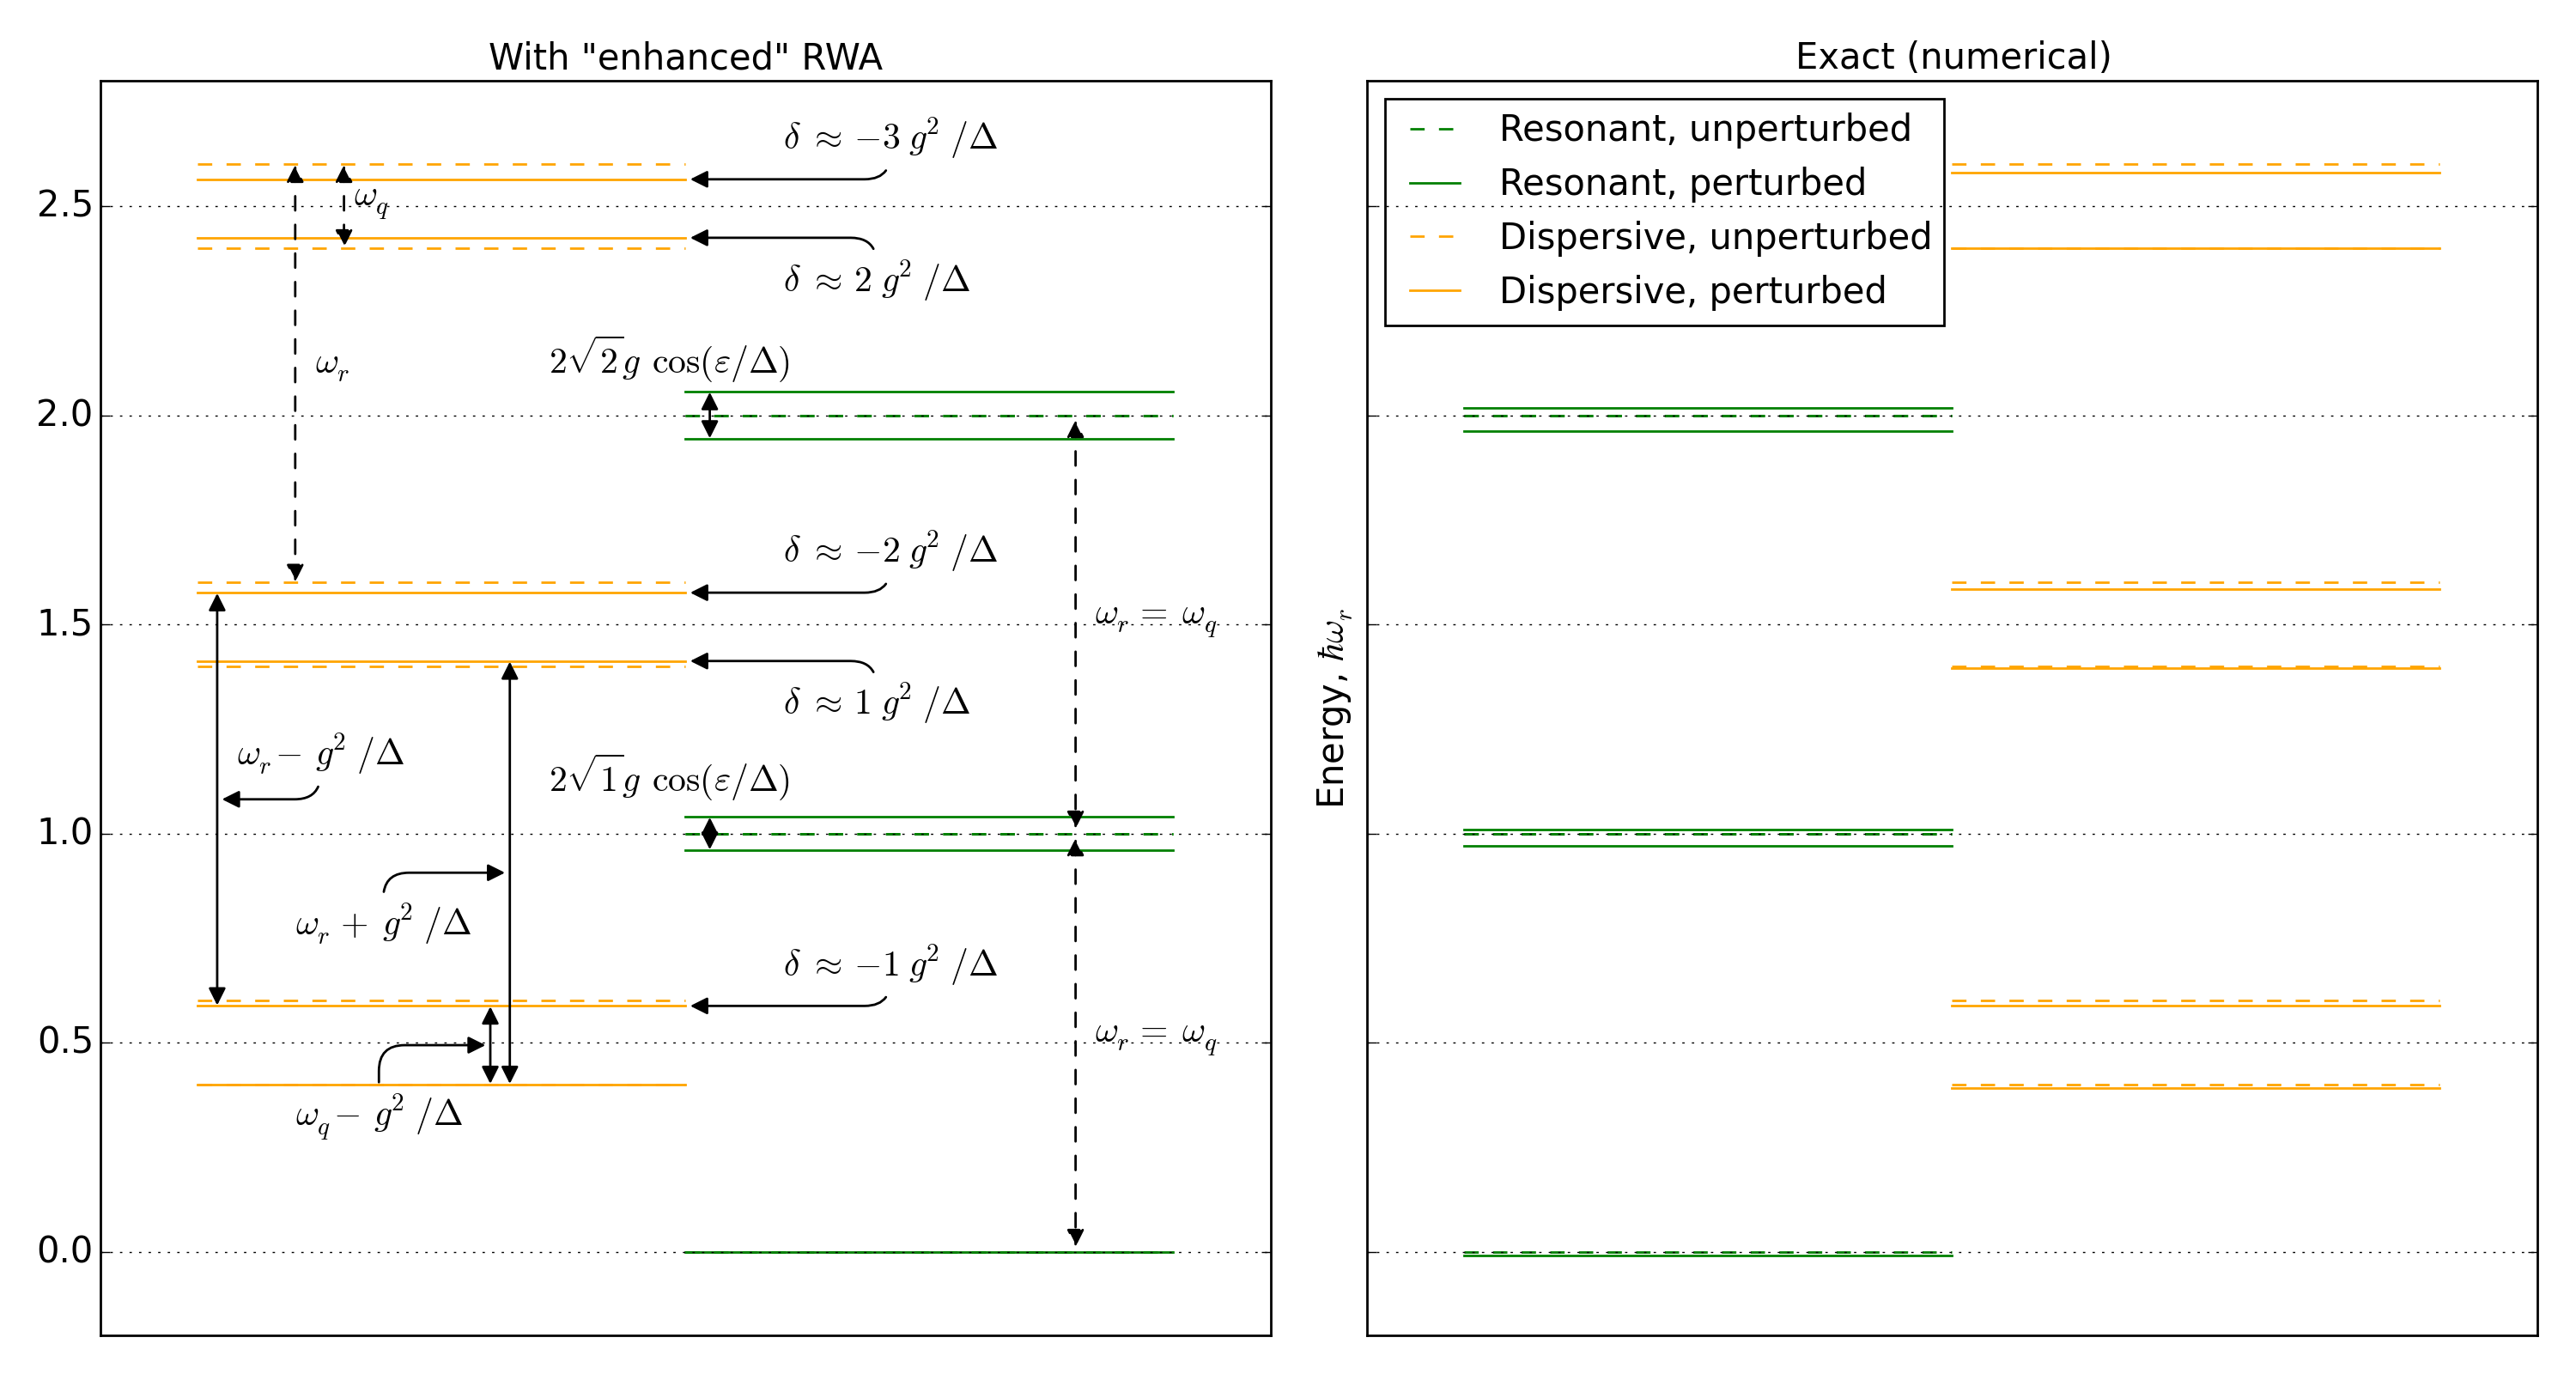
\includegraphics[width=\textwidth]{JCM_levels}
\end{frame}

\begin{frame}[c]\frametitle{\secname}\framesubtitle{\subsecname}
\begin{columns}[c]
\column{0.5\textwidth}
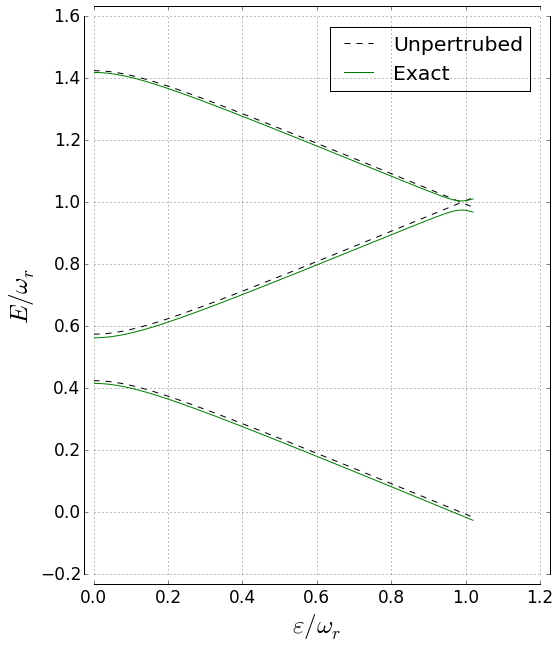
\includegraphics[height=0.85\textheight]{Rabi_levels}
\column{0.5\textwidth}
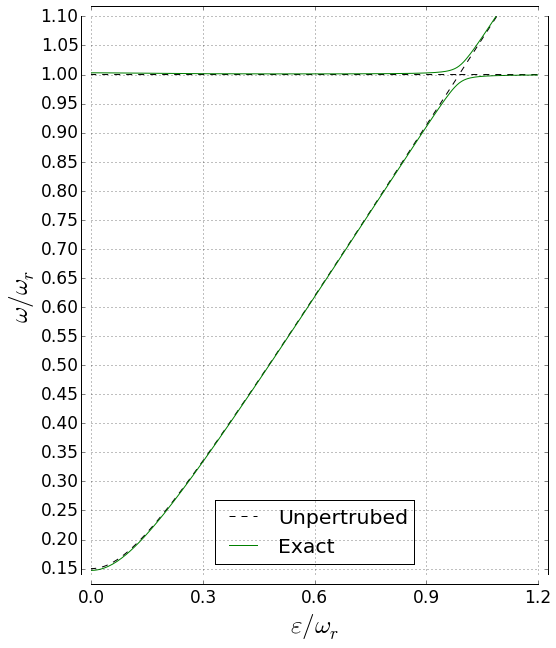
\includegraphics[height=0.85\textheight]{Rabi_spectrum}
\end{columns}
\end{frame}



\subsection{Квазипересечение}
\begin{frame}[c]\frametitle{\secname}\framesubtitle{\subsecname}
\centering
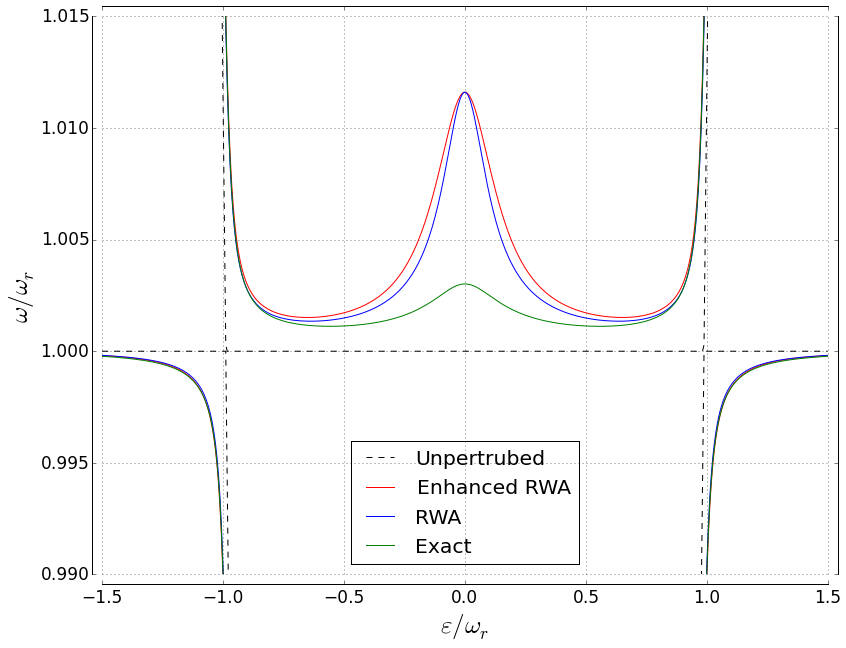
\includegraphics[width=0.7\textwidth]{Rabi_anticrossing}
\end{frame}

\subsection{Основное уравнение и теория отклика}
\begin{frame}[c]\frametitle{\secname}\framesubtitle{\subsecname}
\begin{columns}[c]

\begin{column}{0.5\textwidth}
Основное уравнение форме Линдблада (T $\approx$ 0):
\begin{gather*}
i\hbar \frac{\partial}{\partial t}\hat \rho_s = \sbrkt{\mathcal{\hat H}_s, \hat \rho_s} + \\
+ \sum_{k=1}^3 \Gamma_k \rbrkt{\mathcal{\hat O}_k \hat \rho_s \mathcal{\hat O}_k^\dag - \frac{1}{2} \left\{ \mathcal{\hat O}_k^\dag \mathcal{\hat O}_k, \hat \rho_s \right\} } \\
\mathcal{\hat O}_1 = \hat a,\ \Gamma_1 = \kappa,\\
\mathcal{\hat O}_2 = \hat \sigma^-,\ \Gamma_2 = \gamma, \quad 
\mathcal{\hat O}_3 = \hat \sigma_z,\ \Gamma_3 = \gamma_\phi, \\
\mathcal{\hat H}_s = \mathcal{\hat H}_R + \text{driving}
\end{gather*}
\end{column}


\begin{column}{0.5\textwidth}
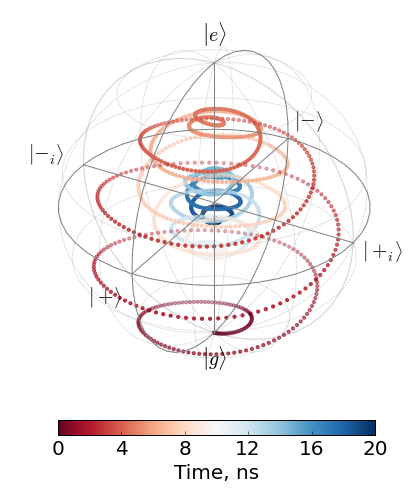
\includegraphics[width=0.9\textwidth]{rabi_dynamics_bloch_rel}
\end{column}
\end{columns}

\end{frame}

\begin{frame}[c]\frametitle{\secname}\framesubtitle{\subsecname}
Теория отклика:
\centering
\begin{equation*}
\mathcal{\hat H}_{tot} = \mathcal{\hat H}_{s} +\int d\omega\ \hbar \omega\, \hat b^\dag(\omega) \hat b(\omega) + \int d\omega\ [ \kappa(\omega) \hat c^{\dag} \hat b(\omega) + \kappa(\omega)\hat c \hat b^{\dag}(\omega)]
\end{equation*}

\begin{columns}[c]
\column{0.5\textwidth}
\begin{block}{Уравнение пропускания}
\centering
$\hat b_{out}= \sqrt{\gamma} \hat c,\quad \hat c \rightarrow \hat a \otimes \mathbbm{\hat 1}_q$\\

\vspace{.5cm}
$S_{21} \propto Tr\left[\hat \rho_s\ \hat a \otimes \mathbbm{\hat 1}_q\right]$
\end{block}
\column{0.5\textwidth}
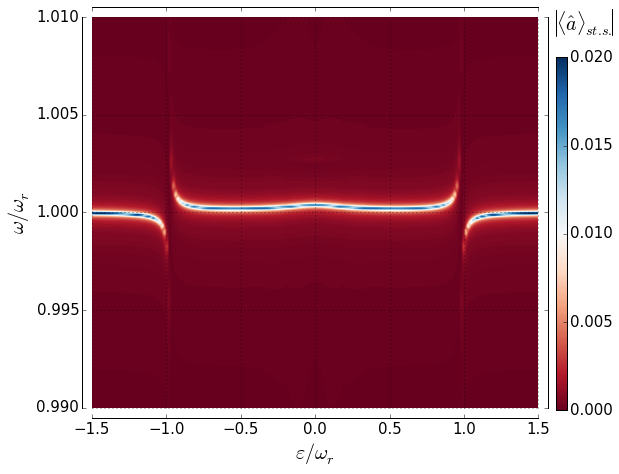
\includegraphics[width=0.9\textwidth]{Rabi_anticrossing_far_dyn}
\end{columns}
\end{frame}


\section{Экспериментальные методы}

\subsection{Образец}
\begin{frame}[c]\frametitle{\secname}\framesubtitle{\subsecname}
\centering
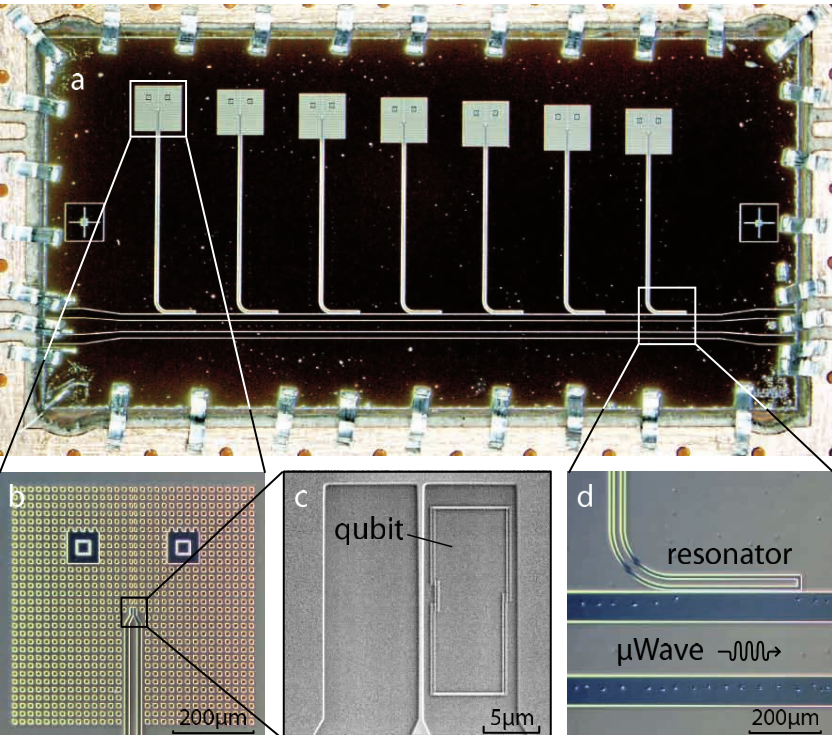
\includegraphics[height=0.8\textheight]{marcus_chip}
\end{frame}

\subsection{Установка}
\frame{\frametitle{\secname}\framesubtitle{\subsecname}
\begin{columns}[c]
\column{\textwidth}
Взаимодействие с образцом внутри криостата:
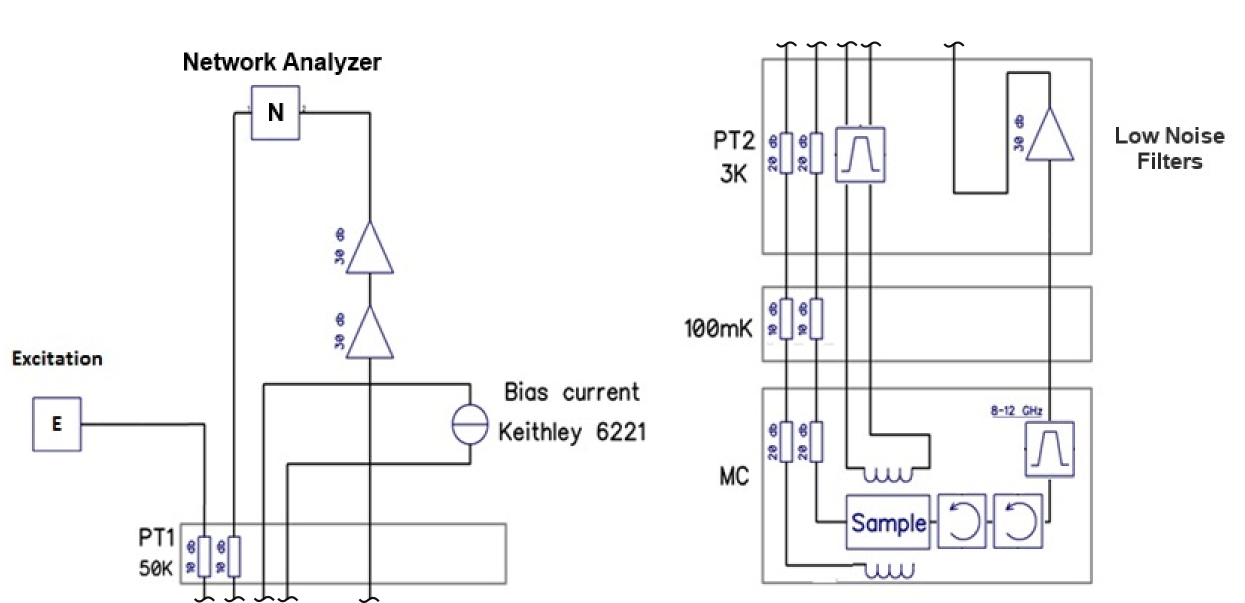
\includegraphics[width=\textwidth]{crio_scheme}
\end{columns}
}
\subsection{Техника измерений}
\frame{\frametitle{\secname}\framesubtitle{\subsecname}
\begin{columns}[c]
\column{0.5\textwidth}

\vspace{-1cm}
В эксперименте фактически наблюдаются сдвиги или расщепления частот поглощения:

\vspace{0.5cm}
\centering
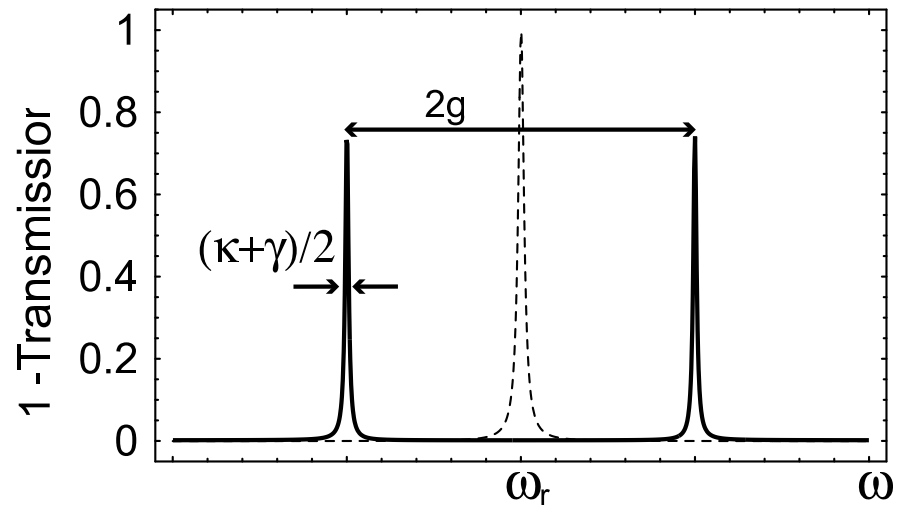
\includegraphics[width=\textwidth]{frequency_shift}
\column{0.5\textwidth}
\centering
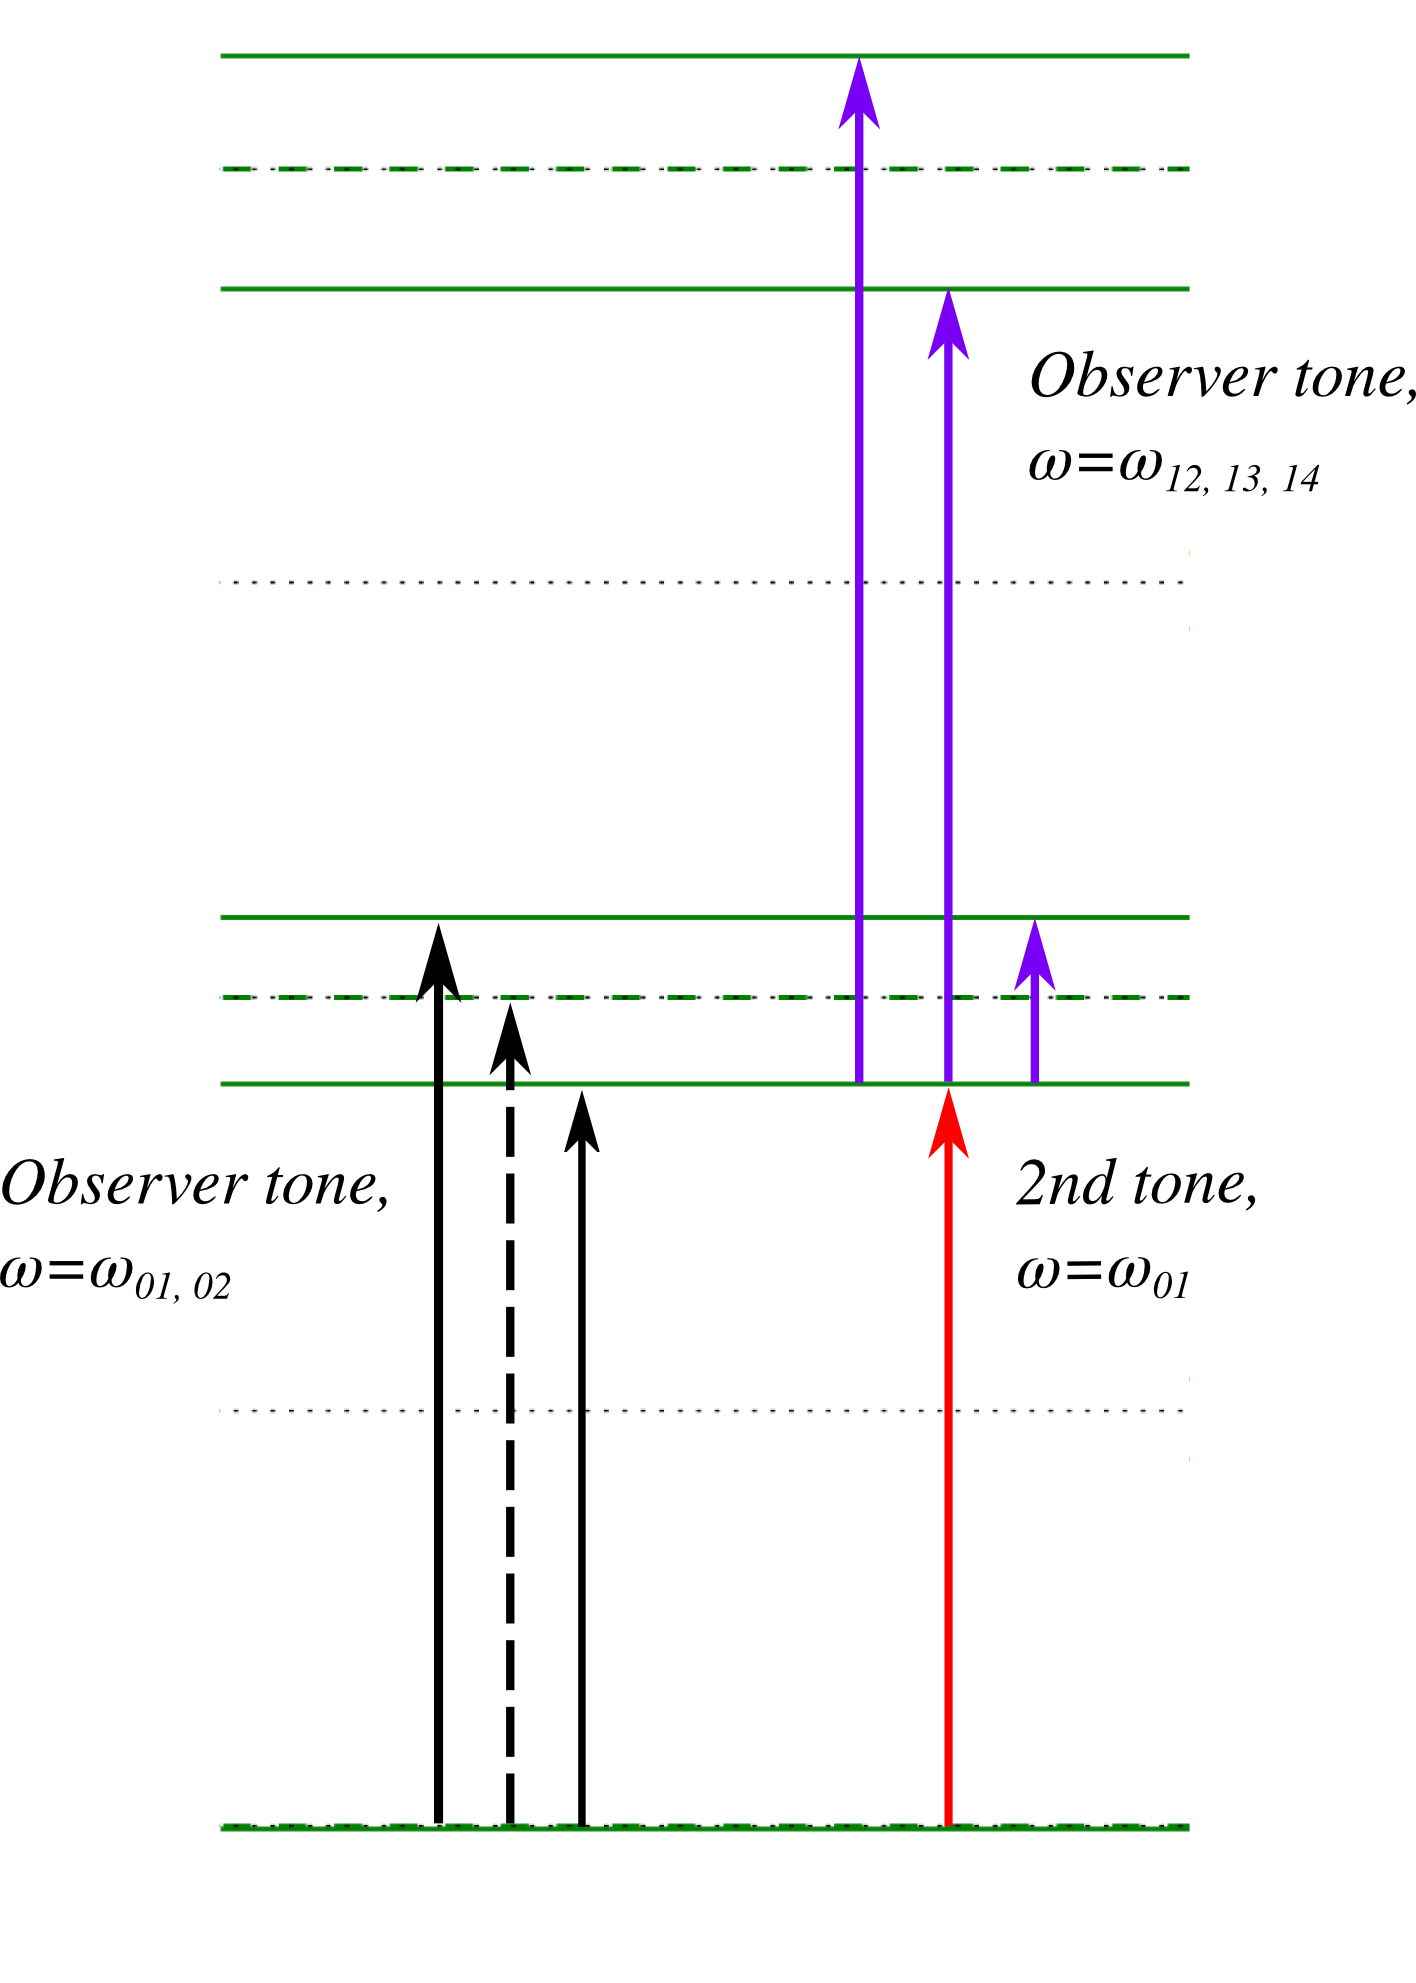
\includegraphics[height=0.85\textheight]{2tone}

\end{columns}
}

\subsection{Двухтоновая спектроскопия}
\begin{frame}[c]\frametitle{\secname}\framesubtitle{\subsecname}
\begin{columns}[c]
\column{0.5\textwidth}
\centering
Теория:

\vspace{1cm}
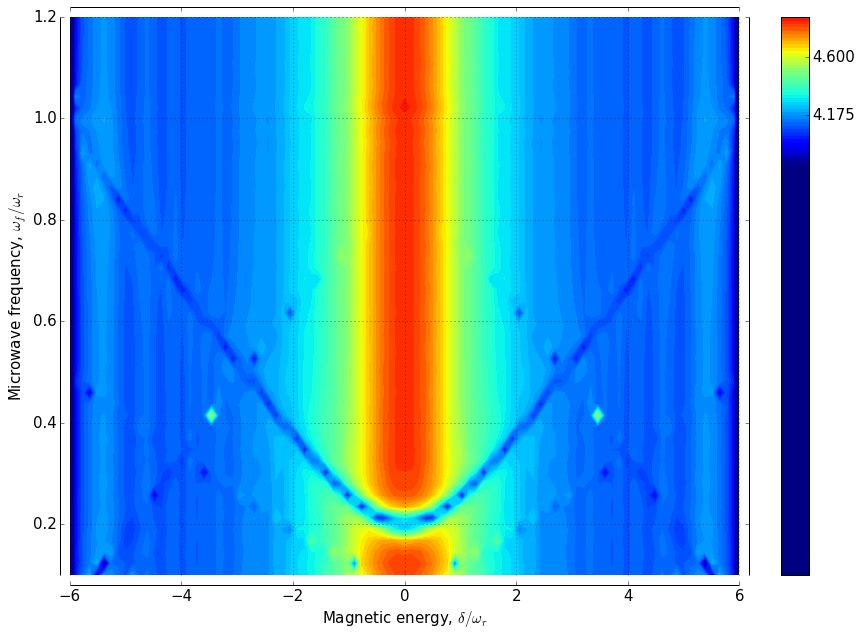
\includegraphics[width=0.9\textwidth]{two_tone_spectrum_numerical}

\column{0.5\textwidth}
\centering
Эксперимент:

\vspace{1cm}
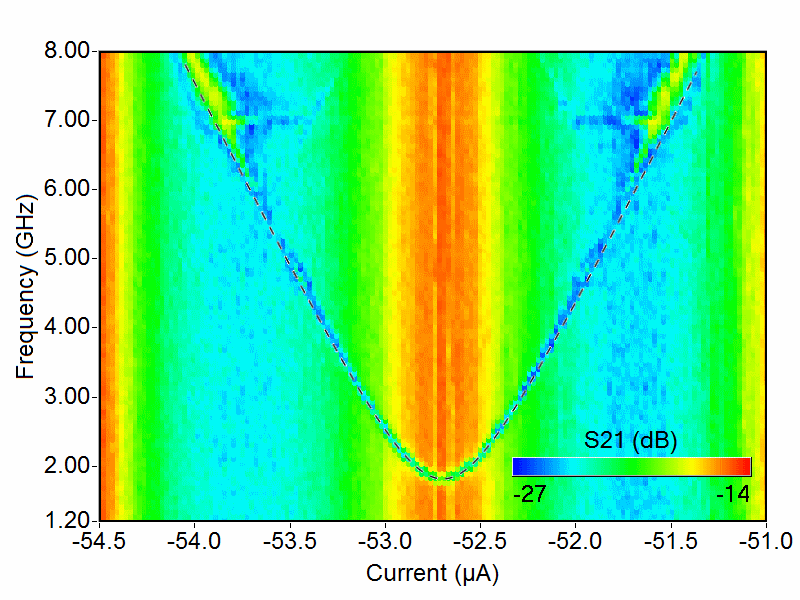
\includegraphics[width=0.9\textwidth]{two-tone_spectrum}

\end{columns}
\end{frame}


\section{Экспериментальные результаты}
\subsection{Спектры}
\frame{\frametitle{\secname}\framesubtitle{\subsecname}

\vspace{0.5cm}
\begin{columns}[t]

\column{0.3\textwidth}
\centering
Второй резонатор

\vspace{0.2cm}
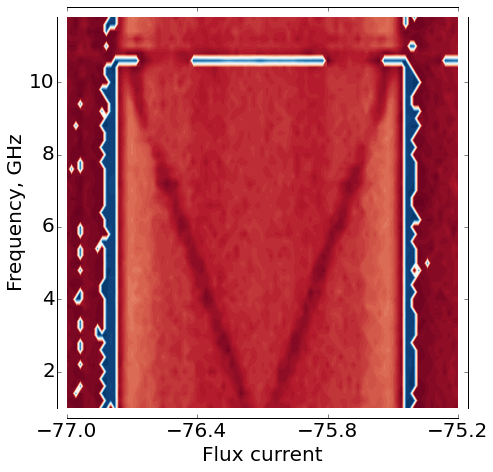
\includegraphics[width=\textwidth]{two-tone_spectrum1}

\column{0.3\textwidth}
\centering
Третий резонатор

\vspace{0.2cm}
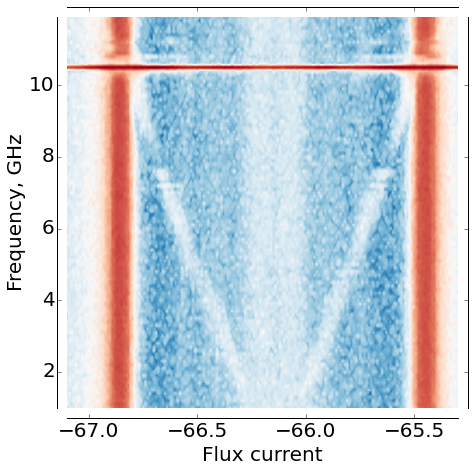
\includegraphics[width=\textwidth]{two-tone_spectrum2}

\column{0.3\textwidth}
\centering
Пятый резонатор

\vspace{0.2cm}
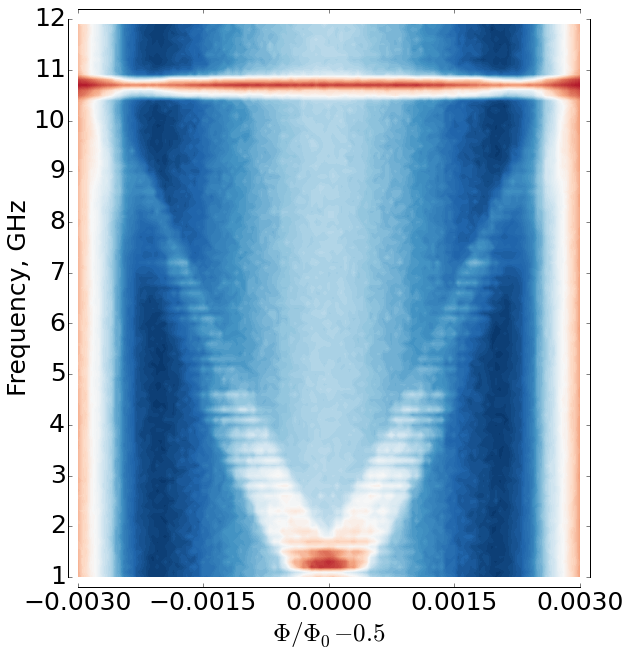
\includegraphics[width=\textwidth]{two-tone_spectrum3}

\end{columns}

\vspace{0.5cm}
Гиперболическая зависимость от $\varepsilon\propto \Phi - \Phi_0/2$:
\centering
\begin{equation*}
\hbar \omega_q = \sqrt{\varepsilon^2+\Delta^2}
\end{equation*}
}
\subsection{Квазипересечение (пятый кубит)}
\frame{\frametitle{\secname}\framesubtitle{\subsecname}
\centering
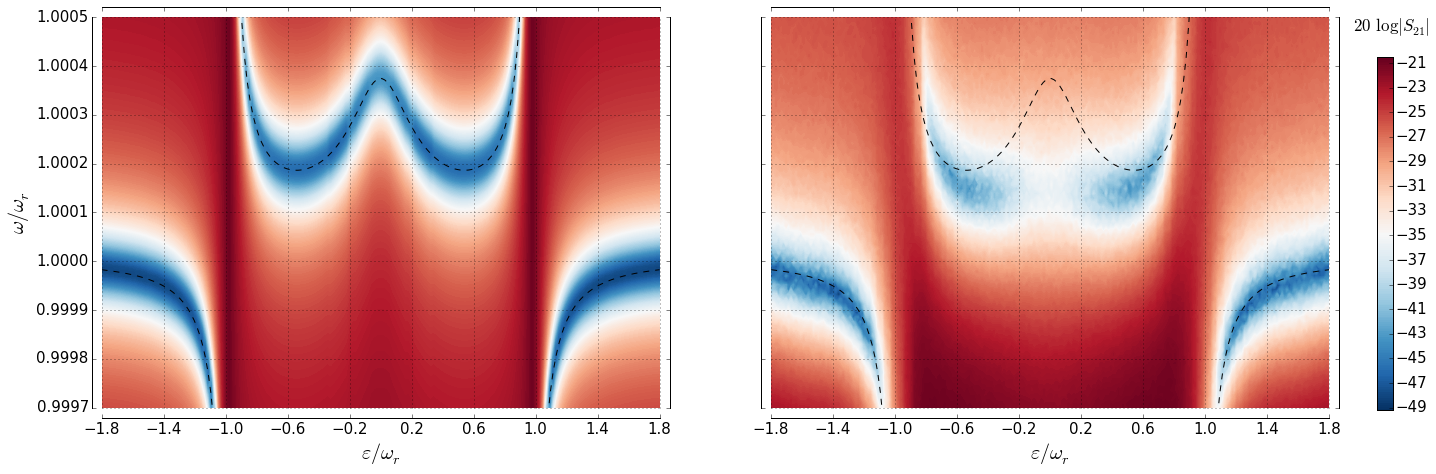
\includegraphics[width=\textwidth]{anticrossing_double}
}
\frame{\frametitle{\secname}\framesubtitle{\subsecname}

\centering
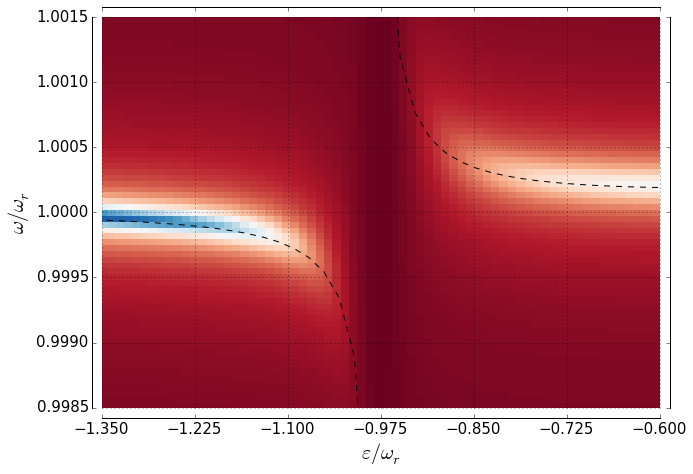
\includegraphics[width=0.5\textwidth]{anticrossing_vanishing} 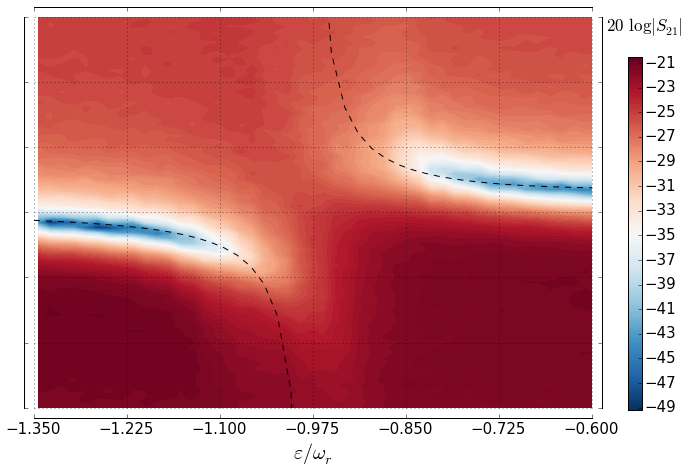
\includegraphics[width=0.5\textwidth]{anticrossing_vanishing_exp}

}

\subsection{Дополнение -- первый отечественный кубит}
\frame{\frametitle{\secname}\framesubtitle{\subsecname}
\centering
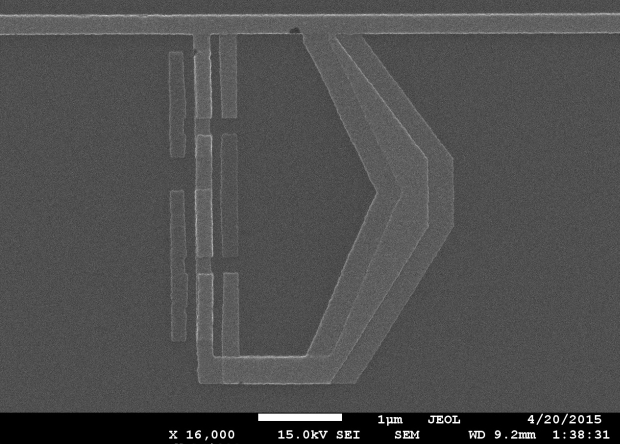
\includegraphics[width=0.7\textwidth]{new_qubit}
}

\frame{\frametitle{\secname}\framesubtitle{\subsecname}
\centering
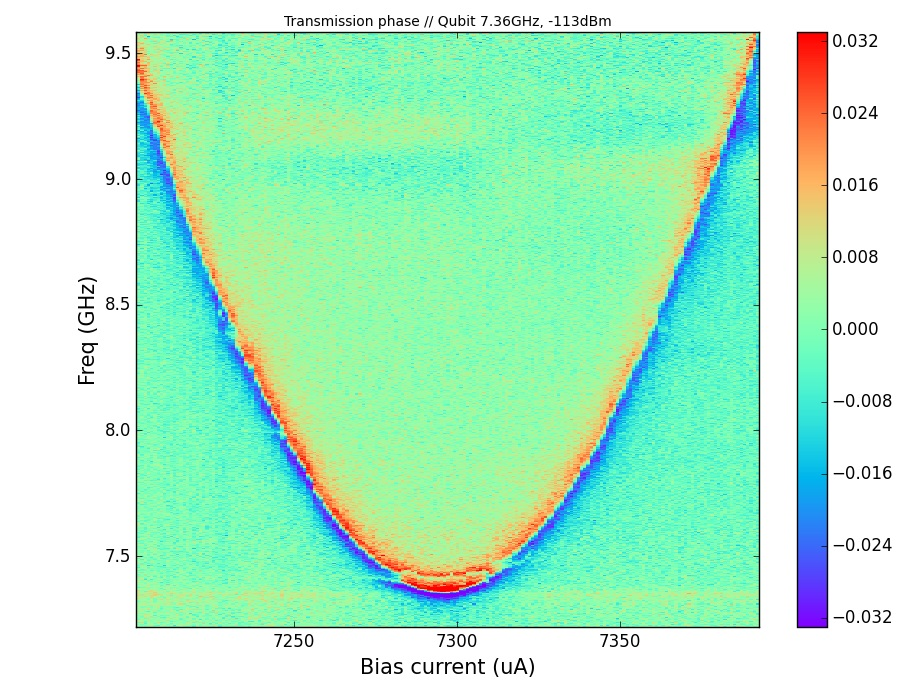
\includegraphics[width=0.7\textwidth]{new_spectrum}
}

\appendix

\section*{Вспомогательные материалы}
\subsection*{Сверхпроводимость и эффект Джозефсона}
\begin{frame}[noframenumbering, c, label=1st]\frametitle{\secname}\framesubtitle{\subsecname}
\addvspace{-2cm}

\begin{columns}[c]
\column{0.5\textwidth}

\vspace{1.2cm}
\only<1>{Теория Г.-Л. и уравнения Джозефсона:}
\only<2>{Квантование магнитного потока:}
\begin{gather*}
\Psi(\mathbf{r}) = \sqrt{\frac{n_s}{2}}e^{i\theta(\mathbf{r})}\\
\only<1>{
I_s = I_c\sin\varphi,\ \hbar\frac{\partial\varphi}{\partial t} = 2eV \\
E = E_J(1-\cos\varphi) + \frac{\hbar^2}{4E_C} \dot \varphi^2, \\ 
E_J = \frac{\hbar}{2e}I_c,\ E_C = \frac{(2e)^2}{2C}
}
\only<2>{
\mathbf{j}_s = \frac{1}{\Lambda}\left(\frac{\Phi_0}{2\pi}\nabla\theta(\mathbf{r})-\mathbf{A}\right)\\
\sum_i \varphi_n = 2\pi\left(\frac{\Phi}{\Phi_0} - k\right),\ k\in \mathcal{Z},\\
\Phi_0 = \frac{h}{2e}
}
\end{gather*}
\column{0.5\textwidth}

\vspace{1cm}
\only<1>{
\centering
Разность фаз на берегах контакта: \\
$\Delta \theta = \varphi$

\vspace{0.2cm}
\hspace{-.2cm}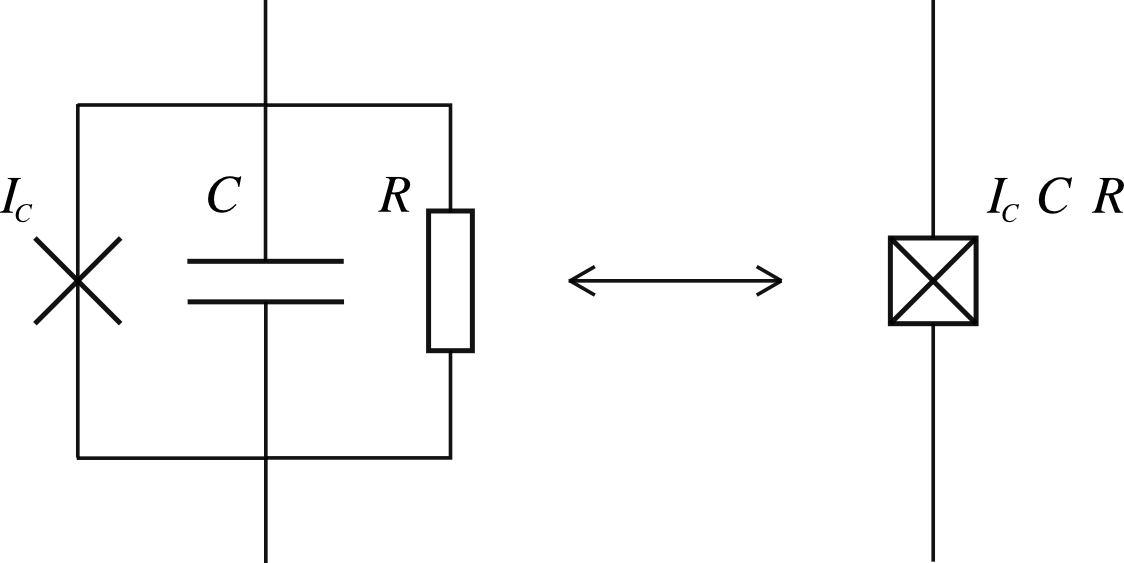
\includegraphics[width=1.05\textwidth]{RCSJ} 

RSCJ-модель
}
\only<2>{\vspace{1cm}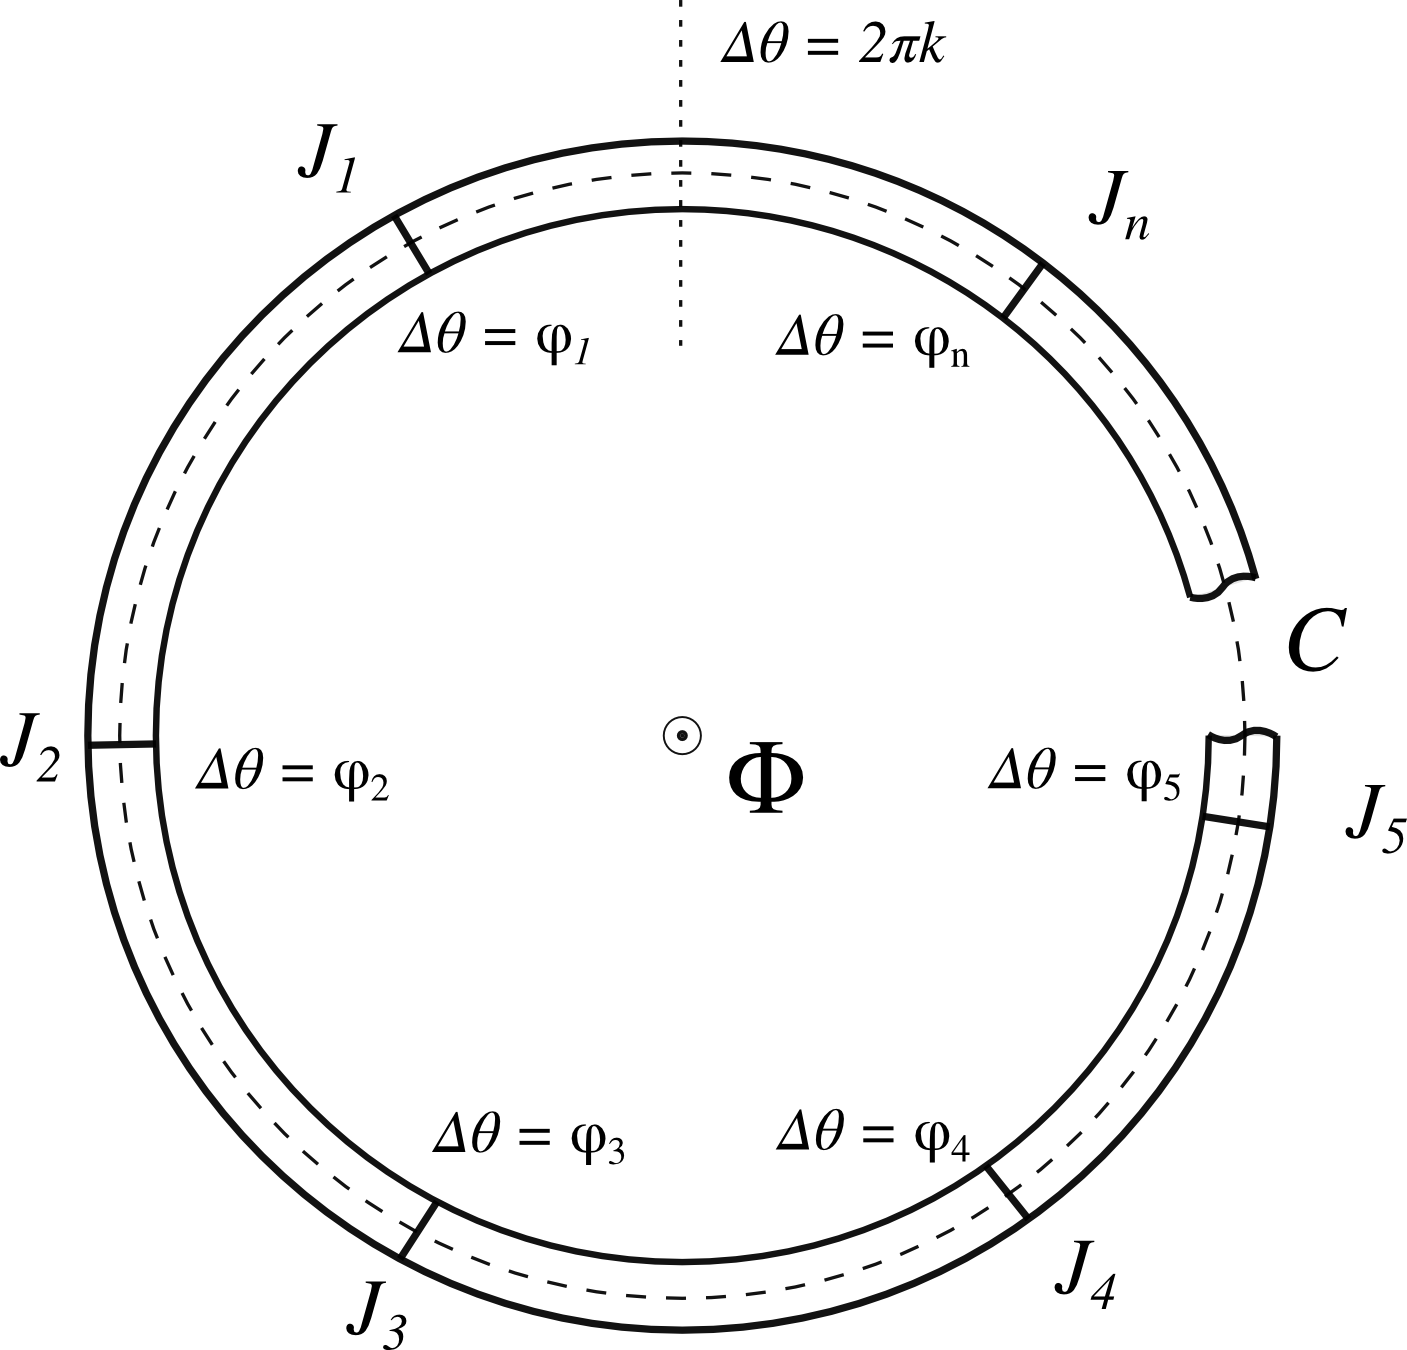
\includegraphics[width=0.9\textwidth]{ring}}
\end{columns}
\end{frame}

\subsection*{Квантовые биты}
\begin{frame}[c]\frametitle{\secname}\framesubtitle{\subsecname}
\begin{columns}[c]
\column{0.5\textwidth}
\centering
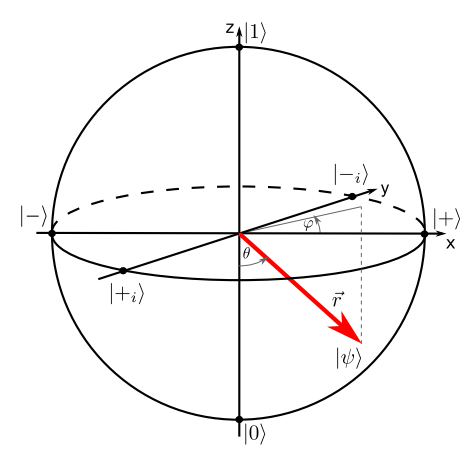
\includegraphics[width=0.85\textwidth]{bloch_sphere}

Сфера Блоха

\column{0.5\textwidth}
Состояние классического бита:
\begin{equation*}
0\ \text{или}\ 1
\end{equation*}
Состояние квантового бита:
\hspace{-2cm}
\begin{equation*}
\ket{\psi} = a\ket{0}+b\ket{1},\ a,b \in \mathbb{C}
\end{equation*}
\end{columns}
\end{frame}



\subsection*{Теория изолированного Flux-кубита}
\begin{frame}[c]\frametitle{\secname}\framesubtitle{\subsecname}

\vspace{-1cm}
\only<1>{

\vspace{0.5cm}
Степени свободы: 
\begin{equation*}
\varphi_1,\ \varphi_2,\ \varphi_3 = 2\pi\frac{\Phi}{\Phi_0} - \varphi_1 - \varphi_2 \ (\text{квантование }\Phi,\ \varphi_3\ \text{зависима от первых двух})
\end{equation*}
}

\only<1>{
\begin{columns}[c]
\column{0.5\textwidth}
Энергия одного перехода:
\hspace{-1cm}
\begin{align*}
E_i = E_J(1-\cos\varphi_i) + \frac{\hbar^2}{4E_C} \dot \varphi_i^2, \\ 
E_J = \frac{\hbar}{2e}I_c,\ E_C = \frac{(2e)^2}{2C}
\end{align*}

\column{0.5\textwidth}
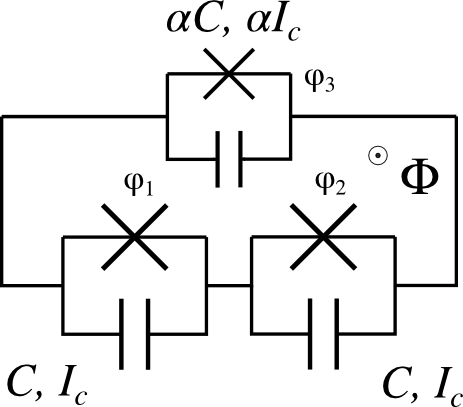
\includegraphics[width = 0.75\textwidth]{qubit}

\end{columns}
}
\only<2>{

\begin{columns}[t]
\column{0.5\textwidth}

\vspace{1cm}
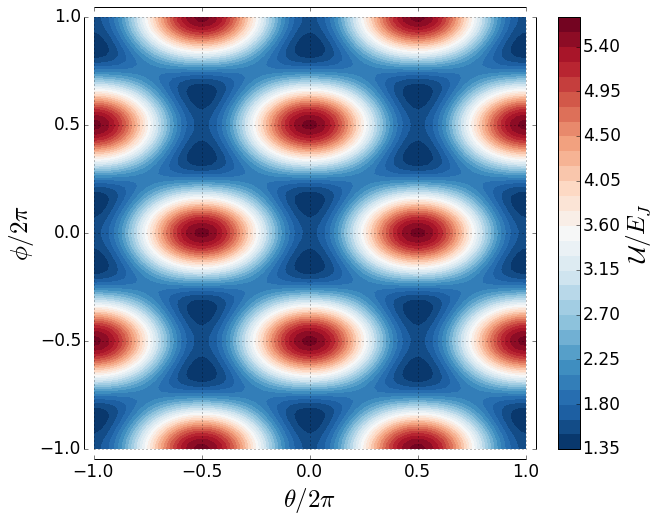
\includegraphics[width=\textwidth]{qubit_potential}

\column{0.5\textwidth}

\vspace{1cm}
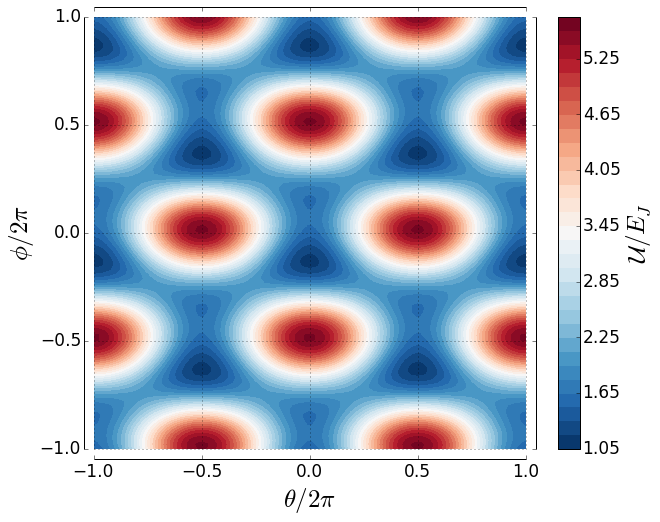
\includegraphics[width=\textwidth]{qubit_potential2}

\end{columns}

\begin{gather*}
 U = E_J\bigg[2+\alpha - 2\cos(\phi)\cos(\theta) 
-\left. \alpha\cos\left(2\pi\frac{\Phi}{\Phi_0} -2\phi \right)\right], \phi = \frac{\varphi_1+\varphi_2}{2}, \theta=\frac{\varphi_1 - \varphi_2}{2}
\end{gather*}
}

\end{frame}

\subsection*{Энергетический спектр Flux-кубита}
\begin{frame}[c]\frametitle{\secname}\framesubtitle{\subsecname}
\only<1>{
\begin{columns}[c]

\column{\textwidth}

\vspace{0cm}
\centering
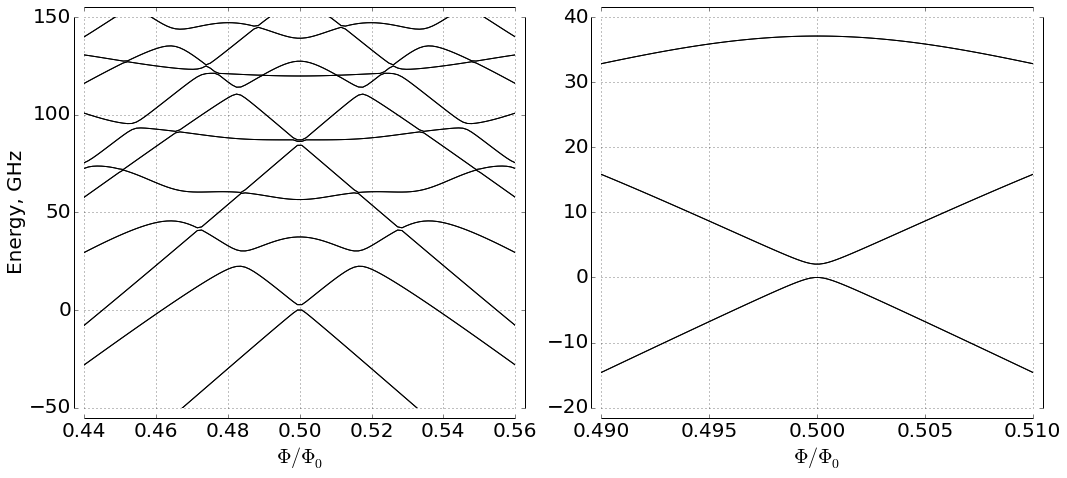
\includegraphics[width=0.7\textwidth]{qubit_levels}
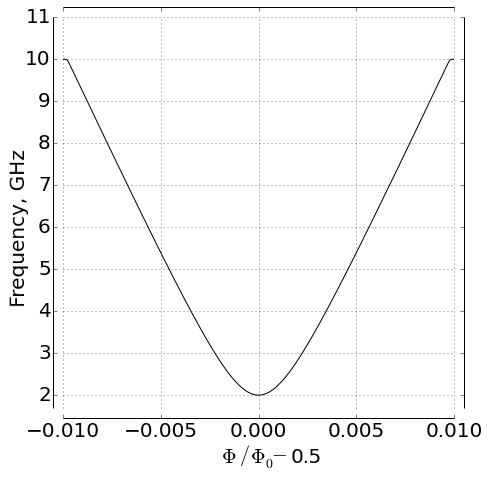
\includegraphics[width=0.307\textwidth]{spectrum_hyp}
\begin{gather*}
\hat{\mathcal{H}} = \frac{\varepsilon}{2}\,\hat\sigma_z + \frac{\delta}{2}\,\hat\sigma_x,\ 
E_1 - E_0 = \sqrt{\varepsilon^2+\delta^2} \text{ -- гипербола по }\delta
 \\ \small{ \ket{0}_{\Phi_0/2}=\rbrkt{\begin{matrix}
1 & 0\end{matrix}}^T,\ \ket{1}_{\Phi_0/2}=\rbrkt{\begin{matrix}
0 & 1\end{matrix}}^T,\ \delta \propto \Phi-\Phi_0/2}
\end{gather*}
\end{columns}
}
\end{frame}



\end{document}